\chapter{Computação em Nuvem}
Apesar do hype \gaaar{hype não é muito técnico} atual da Computação em Nuvem,
o seu conceito não é novo e tão pouco suas técnologias
\cite{CloudUncovered:2012}. Acredita-se que o o conceito de Computação em
Nuvem é o mesmo que John McCarthy, em 1960, se referia a habilidade de prover
e organizar computação como "commodity"\gaaar{aspas são feitas com `` e ''}. 

Este capítulo é dividido em 6 seções, na primeira seção são apresentados as principais definições de computação em nuvem. Na segunda seção são apresentadas suas principais características. Na terceira seção, os modelos de negócio posibilitados pela nuvem são explicados. Na quarta seção é feita uma análise da arquitetura da nuvem. Na quinta seção é feita uma revisão dos os tipos de nuvem. Por fim, na sexta seção os principais desafios da área são apresentados. 


\section{Definição}
	A Nuvem já foi definida de várias formas diferentes. Em \cite{CloudDefinition:2009}, 22  definições diferentes de nuvem são estudadas e, apartir dessas definições, é proposta uma nova definição que contemple as demais:
	
	\begin{quotation}
		"Clouds are a large pool of easily usable and accessible virtualized resources (such as hardware, development platforms and/or services). These resources can be dynamically reconfigured to adjust to a variable load (scale), allowing also for an optimum resource utilization. This pool of resources is typically exploited by a pay-per-use model in which guarantees are offered by the Infrastructure Provider by means of customized SLAs (Service-level agreements)."
	\end{quotation}
	
	A NIST (National Institute of Standards and Technology) em \cite{NIST:2011} define a computação em nuvem abaixo:
	
	\begin{quotation}
		"Cloud computing is a model for enabling ubiquitous, convenient, on-demand network access to a shared pool of configurable computing resources (e. g., networks, servers, storage, applications and services) that can rapidly provisioned and released with minimal management effort or service provider interaction. This cloud model is composed of five essential characteristics, three service models and four deployment models."
	\end{quotation}	
	
	As 5 características essenciais, os 3 modelos de serviço e os 4 tipos de nuvem citados acima, são descritas nas seções seguintes.		

\section{Características}
	Em \cite{NIST:2011} a NIST define que a Computação em Nuvem é composta de cinco características essenciais. Essas características são descritas abaixo:   

\begin{description}

	\item[Auto-atendimento sob demanda:] Um cliente da nuvem pode alocar recursos como processamento e armazenamento, sem que para isso seja necessário qualquer interação humana humana.
	
	\item[Amplo acesso a rede:] Os recursos da nuvem devem estar disponíveis através da rede e podem ser acessados por mecanismos que permitam o acesso por uma gama heterogênea de plataformas como celulares, tablets e notebooks.
	
	\item[Pooling de recursos:] Os recursos computacionais do provedor estão agrupados para servir a multiplos consumidores, utilizando um modelo multi-tenancy, onde diferentes recursos fisicos e virtuais são dinamicamente alocados e desalocados de acordo com a demanda do consumidor. Existe um senso de independência de localização que significa que o consumidor não tem controle nem conhecimento da localização exata dos recursos alocados.
	
	\item[Elasticidade rápida:] Os recursos podem ser elasticamente provisionados, ou seja, quando é necessário mais recursos eles são alocados de forma automática e quando desnecessários esses recursos são desalocados, dando a idéia de que os recursos são ilimitados.
	
	\item[Serviços mensurados:] A nuvem deve ter a capacidade de controlar e otimizar a utilização dos recursos. Dessa forma a utilização dos recursos pode ser monitorada, controlada e reportada, tornando seu uso transparente tanto para o provedor quanto para o consumidor .

\end{description} 



\section{Modelo Negócio}
A computação em nuvem implementa um modelo de negócio orientado a serviços. Em outras palavras, os recursos de hardware e recursos a nível de plataforma são oferecidos como serviços sob demanda. De acordo com \citep{stateOfArt:2010} os serviços oferecidos pelas nuvens podem ser agrupados em três categorias: infrastructure as a service (IaaS), platform as a service (PaaS) e software as a service (SaaS).

\begin{description}

\item[Infrastructure as a Service:] IaaS se refere ao provisionamento sob demanda dos recursos de infraestrutura, normalmente VMs. O dono de uma nuvem que oferece IaaS é chamado de provedor IaaS. Amazon EC2 \cite{AmazonEC2:Online}, GoGrid \cite{GoGrid:Online} e FlexiScale \citep{Aguiar:2005}e{FlexiScale:Online} são exemplos de provedores Iaas.

\item [Platform as a Service:] PaaS se refere ao provisionamento de recursos de plataforma, como sistemas operacionais e frameworks de desenvolvimento de software. Exemplos de provedores PaaS são: Google App Engine \cite{GoogleAppEngine:Online}, Microsoft Windows Azure \cite{MicrosoftAzure:Online} e Salesforce \cite{Salesforce:Online}.

\item[Software as a Service:] Saas se refere ao provisionamento de aplicações sob demanda. Exemplos de provedores SaaS incluem: Rackspace \cite{Rackspace:Online} e SAP Business By Design \cite{SAP:Online}.

\end{description}

O modelo de negócio da computação em nuvem é apresentado na Figura \ref{business-model}. De acordo com a arquitetura em camadas danuvem é totalmente possível que um provedor PaaS funcione sobre um provedor IaaS. Porém o que é muito comum atualmente é que a mesma organização seja o provedor PaaS e IaaS, como a Google e a SalesForce.com. Por esse motivo provedores PaaS e IaaS são frequentemente chamados de provedores de infraestrutura ou provedores de nuvem.

\begin{figure}[htbp]
  \centering 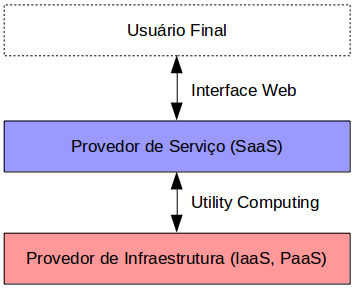
\includegraphics[scale=.6]{imgs/business-model.png}
\caption{Modelo de negócio da computação em nuvem} 
\label{business-model}
\end{figure}


\section{Arquitetura}

Em \citep{stateOfArt:2010} a arquitetura da computação em Nuvem é divida em quatro camadas: a camada de hardware, a camada de infraestrutura, a camada de plataforma e a camada de aplicação, como apresentado na Figura \ref{architecture1}. Que são detalhadas abaixo:

\begin{figure}[htbp]
  \centering 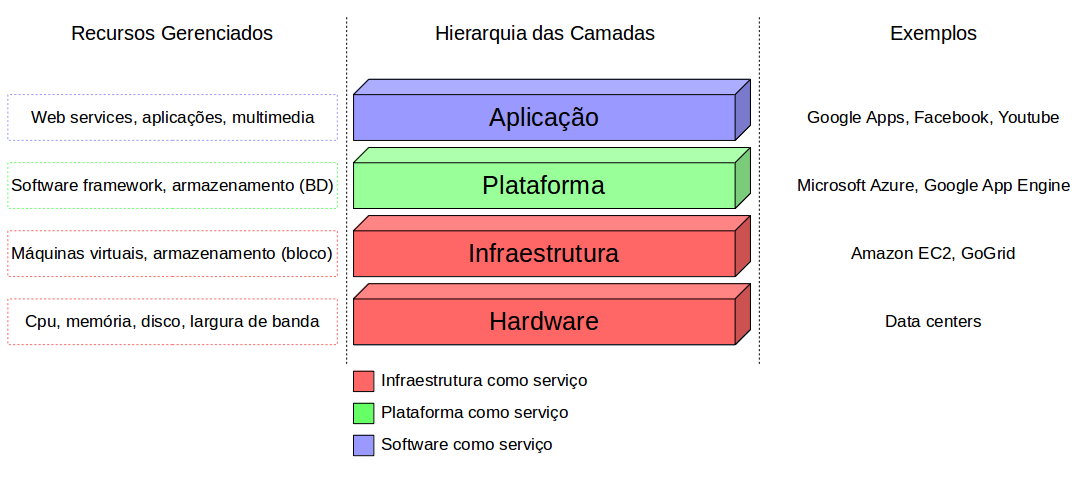
\includegraphics[scale=.4]{imgs/architecture1.png}
\caption{Arquitetura da Computação em Nuvem segundo \citep{stateOfArt:2010}} 
\label{architecture1}
\end{figure}

\begin{description}

	\item[Camada de Hardware:] essa camada é responsável pela gestão dos recursos físicos, incluindo servidores, roteadores, switches, sistemas de resfriamento e energia. Na prática, a camada de hardware é tipicamente implementada nos data centers. Um data center normalmente contem milhares e servidores, que são organizados em racks e interconnectados através de switches ou roteadores. Problemas típicos na camada de harware envolvem configuração de hardware, tolerância a falhas, gerenciamento do tráfego, gerenciamento de energia e gerenciamento dos recursos de resfriamento.

	\item[Camada de Infraestrutura:] também conhecida como camada de virtualização, a camada de infraestrutura cria uma pool de armazenamento e recursos computacionais através do particionamento dos recursos físicos utilizando técnologias de virtualização como Xen \cite{Xen:Online}, KVM \cite{KVM:Online} e VMware \cite{VMware:Online}. Como as principais features da computação em nuvem, como alocação dinâmica de recursos, só são possíveis por causa das tecnologias de virtualização, a camada de infraestrutura é considerada um componente essencial na arquitetura.

	\item[Camada de Plataforma:] contruida sobre a camada de infraestrutura, a camada de plataforma consiste em sistemas operacionais e frameworks. O propósito da camada de plataforma é facilitar o deploy[tradução?] de aplicações em máquinas virtuais. Por exemplo o Google App Engine opera na camada de plataforma provendo uma API com suporte para armazenamento e lógica de negócio para aplicações web típicas. 

	\item[Camada de Aplicação:] no level mais alto da hierarquia, a camada de aplicação consiste nas aplicações da nuvem. Diferentes das aplicações tradicionais, as aplicações da nuvem fazem uso da feature de escalonamento-automático para alcançar uma melhor performace, disponibilidade e baixo custo de operação.

\end{description}

Comparado aos ambientes de hospedagem de serviços tradicionais como servidores dedicados, a arquitetura da nuvem é mais modular. Cada camada é fracamente acoplada, com camadas acima e abaixo, permitindo que cada camada evolua separadamente. Essa modularidade permite que a computação em nuvem de suporte a uma gama de requerimentos das aplicações enquanto reduz o overhead de manutenção e de administração.

Em \citep{demystifingCloud:2011} a arquitetura também é dividida em quatro camadas com uma hierarquia baseada na abstração, porém a arquitetura é definida diretamente ligada aos modelos de negócio, como pode ser observado na Figura \ref{architecture2}. Nessa definição é adicionando um novo modelo de negócio: dados como serviço, que é descrito como o serviço que oferece base de dados para armazenamento das informações do cliente. 

\begin{figure}[htbp]
  \centering 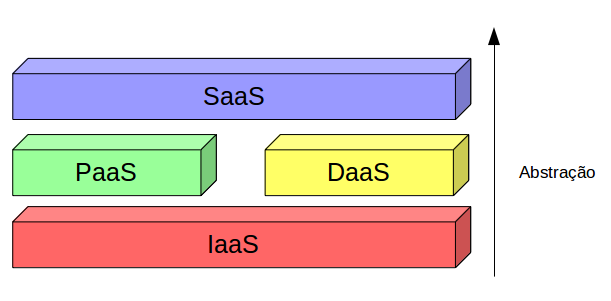
\includegraphics[scale=.6]{imgs/architecture2.png}
\caption{Arquitetura da Computação em Nuvem segundo \citep{demystifingCloud:2011}} 
\label{architecture2}
\end{figure}

\section{Tipos de Nuvem}

	Em \citep{stateOfArt:2010} e \cite{NIST:2011} 4 tipos de nuvem são descritos: Nuvem Pública, Nuvem Privada, Nuvem Híbrida e Nuvem Comunitária.

	\begin{description}
	
		\item[Nuvem Pública:] nuvem onde os provedores de serviços oferecem seus recursos como serviços ao público geral. Nuvens publicas oferecem vários benefícios aos provedores de serviço, por exemplo, não é necessários para os provedores investimentos inciais em infraestrutura. No entanto, as nuvens públicas oferecem um baixo grau de controle sobre os dados, a rede e as configurações de segurança.  	 
			
		\item[Nuvem Privada:] também conhecida como nuvem interna, as nuvens privadas são para uso exclusivo de uma organização. A nuvem privada pode ser construida e gerenciada pela própria empresa ou por provedores externos. Esse tipo de nuvem oferece um maior controle de performace, segurança e confiabilidade. No entanto, as nuvens privadas são criticadas por serem muito similares aos servidores tradicionais.
		
		\item[Nuvem Híbrida:] uma nuvem híbrida é a combinação da nuvem privada e da nuvem pública, na tentativa de minimizar as limitações das duas abordagens. Nesse tipo de nuvem, parte dos serviços de infraestrutura estão na nuvem privada enquanto que as outras partes são executadas em uma nuvem pública. Nuvens hibridas oferecem mais flexibilidade que as nuvens públicas e do que as nuvens privadas. Elas oferecem mais controle sobre dados, rede e segurança do que as nuvens públicas mantendo as facilidades de expansão.
		
		\item[Nuvem Comunitária:] a nuvem comunitária funciona praticamente como uma nuvem privada que pode ser utilizada por duas ou mais organizações. Ela pode ser gerenciada tanto por uma organização, pelas duas organizações, ou por um provedor.
		 	
	\end{description}
	
\section{Desafios}

	Apesar da Computação em Nuvem estar amplamente presente na indústria, as pesquisas nesta área ainda estão em fase inicial \cite{stateOfArt:2010}.  Muitos problemas existentes ainda não foram resolvidos, enaquantos novos desafios continuam surgindo das aplicações nas indústrias. Essa seção apresenta um resumo dos principais desafios da Computação em Nuvem. 
	
	\subsection{Provisionamento Automático de Serviço}
	Umas das principais características da Computação em Nuvem é a capacidade de adquirir e liberar recursos sob demanda. O objetivo de um provedor de serviço neste caso é de alocar e desalocar recursos da nuvem a fim de satisfazer os service level objectives (SLOs), enquanto minimiza o custo operacional.  No entanto, não é óbvio como o provedor de serviço alcançará esse objetivo. Em particular, não é fácil de determinar como mapear SLOs tais como requisitos de QoS para requisitos dos recursos de baixo nível como requisitos de CPU e de memória. Além disso, para alcançar alta agilidade para responder as flutuações de demanda, as decições de provisionamento devem ser feitas em tempo real.
	
	\subsection{Migração de Máquinas Virtuais}
	A virtualização é uma das principais tecnologias utilizadas em infraestruturas em nuvem. Através do uso da virtualização, é possível compartilhar a mesma máquina física com múltiplos sistemas operacionais e/ou aplicações de usuários finais, promovendo o isolamento entre os mesmos. Da mesma forma, o seu uso torna possível realizar balanceamento de carga entre estruturas físicas, através de ações como a migração de máquinas virtuais entre servidores.
	
	A migração de VMs evoluiu das técnicas de migração de processos \cite{Osman:2002}. Algumas ferramentas já implementam o conceito de live-migration, onde as VMs são movidas em um processo que envolve paradas extremamente curtas que variam de dezenas de milissegundos a um segundo. Clark et al. \cite{Clark:2005} mostra que a migração de um SO inteiro e todas suas aplicações como uma unidade permite que muitas das dificuldades encontradas nas abordagens de migração de processos sejam evitadas.
	 
	O maior benefício da migração de VMs é a capacidade de evitar a sobrecarga de pontos específicos da infraestrutura de servidores, no entanto essa não é uma tarefa simples. Atualmente, a detecção de pontos de sobrecarga e o disparo de uma migração não tem agilidade suficiente para responder às mudanças de carga de trabalho repentinas. Além disso, é necessário transferir o estado dos dados em memória de forma consistente e eficiente, considerando os recursos para as aplicações e para os servidores físicos. 
	
	\subsection{Consolidação de Servidores}
	A consolidação de servidores é uma abordagem que tem como objetivo maximizar a utilização de recursos enquanto minimiza o consumo de energia. A técnica de migração de VMs é frequentemente utilizada na consolidação de servidores, onde VMs são movidas de multiplos servidores sub-utilizados para um servidor. Dessa forma os servidores restantes são colocados no estado de economia de energia. O problema de consolidar servidores de forma ótima pode ser visto como uma variação do problema bin-packing \cite{Chekuri:1999}, que é um problema de otimização NP-dificil.
	
	\subsection{Gerenciamento de Energia}
	Atingir uma maior eficiência no consumo de energia também é um dos principais desafios da computação em nuvem. Em \cite{Hamilton} foi estima que o custo de powering(tradução) e refrigeração somam 53 por cento dos gastos operacionais dos data centers. Em 2006, os data centers nos Estados Unidos consumiram mais de 1.5 porcento de toda energia gerada naquele ano, e o crescimento dessa porcentagem tem projeção de crescimento de 18 porcento ao ano. O que leva a uma enorme pressão sobre os provedores de infraestrutura à reduzir o consumo energético. O Objetivo não é apenas reduzir o gasto energético, mas também se adequar aos regulamentos do governo e as normas ambientais. 
	
	\subsection{Segurança dos Dados}
	A segurança dos dados é outro tópico de pesquisa muito importante na computação em nuvem. Visto que os provedores dos serviços tipicamente não têm acesso aos sistemas de segurança dos data centers, eles dependem do provedor de infraestrutura para garantir a segurança de seus dados. Os provedores de infraestrutura devem garantir:
	\begin{description}
		\item[Confidencialidade] para as transfêrencias e acessos a dados.
		\item[Auditabilidade] para atestar se as configurações de segurança de uma aplicação foram modificadas ou não.  
	\end{description}	 
	
	Confidencialidade é normalmente alcançada utilizando protocolos de criptografia, enquanto que a auditibilidade é alcançada utilizando técnicas de atestado remoto. Atestados remotos tipicamente necessitam de um trusted platform module (TPM) para gerar um sumário do sistema infalsificável como prova da segurança do sistema. Porém num ambiente como a nuvem onde as VMs podem migrar dinâmicamente de um servidor para outro, utilizar atestado remoto não é o suficiente. É necessário que seja criado um mecânismo confiável em cada camada da arquitetura. Inicialmente, para ser confiável, a camada de hardware deve usar um TPM. A camada de infraestrutura, resposável pela migração das VMs, deve utilizar monitores de VMs confiáveis. A migração de VMs só deve ser permitida se tanto o servidor de destino quanto fonte são confiáveis.


